\documentclass{article}

\usepackage{polski}
\usepackage[utf8]{inputenc}
\usepackage{graphicx}
\usepackage{url}
\usepackage{amsmath}

\newcommand{\bb}{\textbf}


\title{Praca inżynierska}
\date{2017-10-01}
\author{Jędrzej Kozal, Karol Szpila}

\begin{document}

\begin{titlepage}
	\centering
	
\includegraphics[width=0.25\textwidth]{logo_pol_wroclaw.png}\par\vspace{1cm}
	{\scshape\LARGE Politechnika Wrocławska \par}
	\vspace{1cm}
	{\scshape\Large Sieci neuronowe i neurosterowniki \par}
	\vspace{1.5cm}
	{\huge\bfseries Sprawozdanie z projektu \par}
	\vspace{2cm}
	{\Large\itshape Michał Leś, Jędrzej Kozal\par}
	\vfill
	prowadzący\par
	Dr ~Piotr \textsc{Ciskowski}

	\vfill

% Bottom of the page
	{\large 2017-10-01\par}
\end{titlepage}

\section{Wstęp}
Podstawowym założeniem projetku jest zaznajomienie się z neurosterownikami, ich zasadami działania oraz przygotowanie modelu predykcyjnego prostego obiektu dynamicznego. Dodatkowo przyjęto że bardziej interesujące będzie przyjęcie jakiegoś rzeczywistego obiektu niż badanie reakcji na teoretyczne charakterystyki jakie mogą posiadać obiekty.

Neurosterowniki są sposobem zaadresowania w Automatyce kwestii sterowania obiektami mocno nieliniowymi, z którymi tradycyjne metody sterowania jak sterowniki PID nie dają sobie rady. U podstaw działania neurosterowników leży idea działania sieci neuronowej, które ostatnio zdominowały pole uczenia maszynowego. Są one wykorzystywane w wielu dziedzianach nauki i techniki do rozpoznawania obrazów (computer vision), klasyfikacji, sterownia ruchem ulicznym, wspomagania użytkowników różnych aplikacji (jak np. podpowiadanie słów w trakcie pisania na smarphonie), czy nawet eksperymenty społeczne. W nimniejszej pracy postawiono zbadać w jaki sposób szerokie możliwości oferowane przez sieci neuronowe mogą być wykorzystane w automatyce.

\section{Podstawy teoretyczne}

\subsection{Przyjęty model obektu}

Obiekt w automatyce jest traktowany jako czarna skrzynka, która posiada wejścia i wyjścia. Na pobudzenie na wejściu reaguje odpowiedzią na wyjściu. Odpowiedź systemów dynamicznych zależy nie tylko od aktualnej wartości wejścia, ale także statnu obiektu w poprzednich chwilach. Zgodnie z tym można zapisać model nieliniowego obiektu dynamicznego jako:

\begin{equation}
\left\{
\begin{array}{ll}
	\bb{x}(k+1) &= \phi (\bb{x}(k), \bb{u}(k)) \\
	\bb{y}(k)   &= \psi (\bb{x}(k))
\end{array} \right.
\label{rownanie_stanu}
\end{equation}

Układ \ref{rownanie_stanu} przedstawia równania stanu. Pierwsze równanie wiąże wewnętrzny stan obiektu z pobudzeniem, a drugie równanie wiąże stan obiektu z wyjściem. System opisywany tymi równaniami jest niezmienny w czasie (angl. time-invariant) - $\phi$ i $\psi$ nie zależą bezpośrednio od czasu.

Jeśli zastąpimy funkcje nieliniowe przez odpowiednie macierze zyskamy system liniowy:

\begin{equation}
\left\{
\begin{array}{ll}
	\bb{x}(k+1) &= A\bb{x}(k) + B\bb{u}(k) \\
	\bb{y}(k)   &= C\bb{x}(k) + D\bb{u}(k)
\end{array} \right.
\end{equation}

W rzeczywistych systemach w równaniach oprócz stanu $x$ i pobudzenia $u$ pojawiają się także zakłócenia $z$, które nie będą tutaj rozważane.

Klasa systemów liniowych jest od dawna dobrze znana. Znaleziono wiele sposobów badania i algorytmów sterowania obiektami liniowymi. O wiele trudniejsze w sterowaniu są obiekty nieliniowe. Nawet znając funkcję $\psi$ oraz $x(k)$ samo stworzenie modelu mogącego dokonać identyfikacji takiego obiektu jest trudne, ze względu na kumulujące się z czasem błędy numeryczne, oraz poprzez konieczność poczynienia założeń co do stabilności systemu.

Najprostsza reprezentacja systemu dynamicznego nie zawiera wewnętrznego stanu, który w wielu wypadkach może być pominięty

\begin{equation}
	\bb{y}(k+1) = f(\bb{y}(k),\bb{u}(k))
\end{equation}

\subsection{Zadanie identyfikacji obiektu}

Zadanie identyfikacji sprowadza się do wyznaczeniu modelu reagującego na poubudzenie w sposób zbliżony do reakcji rzeczywistego obietku:

\begin{equation}
	|| \hat{y} - y || < \epsilon
	\label{warunek}
\end{equation}

\begin{figure}
\centering
	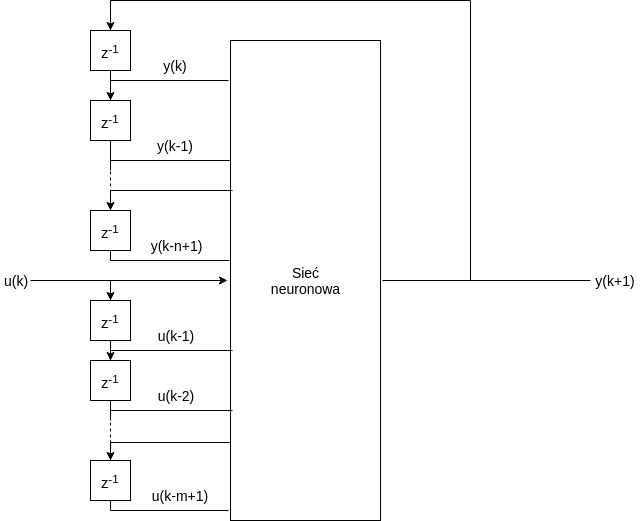
\includegraphics[width=0.90\textwidth]{ident.jpg}\par\vspace{1cm}
\caption{Model identyfikacji obiektu z wykorzystaniem sieci neuronowej.}
	\label{fig:identyfikacja}
\end{figure}

Uzyskanie takiego modelu umożliwia sterowanie adaptacyjne, co znacznie ułatwia pracę z obiektami nieliniowymi. Celem sterowania w ogólności jest uzyskanie na wyjściu obiektu $\bb{y}(k)$ wartości jak najbardziej zbliżonoej do wartości zadanej $\bb{y}_m(k)$. W przypadku sterowania adaptacyjnego oznacza to znaleznie takiego pobudzenia $\bb{u}(k)$ aby została spełniona zależność:

\begin{equation}
	\displaystyle{\lim_{k \to \infty}} ||\bb{y}(k)-\bb{y}_m(k)|| < \epsilon
\end{equation}

Często do takiego zadania są wykorzystywane sieci neuronowe przedstawione na rys. \ref{fig:identyfikacja}. Na wejście sieci podaje się wejścia systemu, oraz wyjścia z poprzednich chwil. Zadaniem sieci jest przewidzenie zachowania systemu w kroku $k+1$. Szereg bloków opóźniających będzie dalej oznaczany w pracy jako TDL(Tapped Dleay Line).

\begin{figure}
\centering
	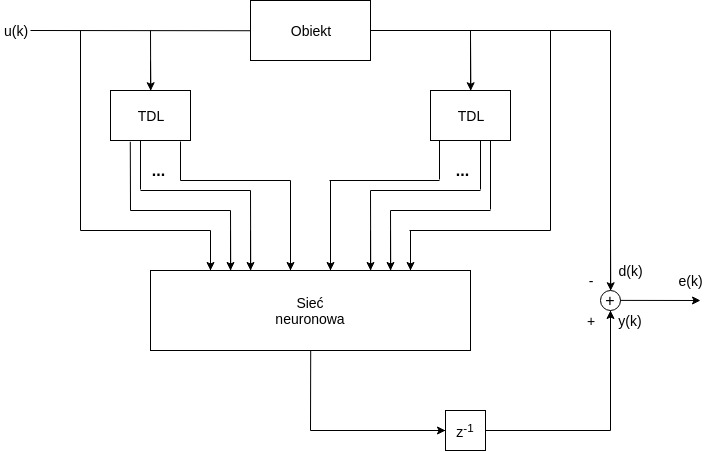
\includegraphics[width=0.90\textwidth]{ident2.jpg}\par\vspace{1cm}
\caption{Schemat podłączenia sieci neuronowej w trakcie uczenia.}
	\label{fig:identyfikacja2}
\end{figure}

W trakcie identyfikacji sieć neuronowa jest zwykle włączana sposób szeregowo-równoległy, co zostało zilustrowane na rys \ref{fig:identyfikacja2}. Taka konfiguracja umożliwia badanie błędu i minializację błędu zgodnie z nierównością \ref{warunek}. Sieć neuronowa nieustanie próbuje przewidzieć wyjście obiektu w następnej chwili. Różnica $e(k)$ jest wykorzystywana w procesie uczenia sieci. W \cite{Osowski} zaproponowano taką metodę oraz zaprezentowano wykorzystanie modelu do predykcji wyjścia filtru Butterwortha szóstego rzędu dla pobudzenia sygnałem trójkątnym oraz tłumionym sygnałem sinusoidalnym.

\section{Zrealizowane zadania oraz otrzymane wyniki}
Zadanie predykcji może zostać zrealizowane za pomocą modelowania liniowego ARX -
modelu auteregresywnego z zewnętrznym wejściem. Jeżeli do modelowania zostały
użyte sieci neuronowe model taki nazywa się NNARX (Neural Networ ARX).

Na podstawie danych zawartych w pliku 'actuator.m' żądany model został załadowany
do środowiska programu Matlab. Wejściem obiektu (u) jest
otwarcie zaworu, zaś odpowiedzią systemu(y) jest ciśnienie oleju.
Pierwszym elementem potrzebnym do wykonania zadania była konstrukcja prawidłowego ciągu uczącego.
W modelu ARX potrzebujemy stworzyć układ z opóźnionymi wejściami i odpowiedziami.
W zależności od potrzeb modelu, możemy dostosować wielkość opóźnienia i ilość opóźnionych próbek.
W naszym przypadku skonstruowana została następującą macierz wejściowa dla sieci:
\begin{equation}
	u_s= \begin{bmatrix} 0 & 0 & 0 & 0 \\ 0 & u' & 0 & 0 \\ 0 & 0 & u' & 0 \\ 0 & p' & 0 & 0 \\ 0 & 0 & p' &  0 \\ 0 & 0 & 0 & p' \end{bmatrix}
\end{equation}
gdzie u' i y' odpowiadają transponowanym wektorom otrzymanym z modelu.
Analogicznie skonstruowany został wektor pożądanych wyjść dla sieci:
\begin{equation}
	y_s= \begin{bmatrix} p' & 0 & 0 & 0  \end{bmatrix}'
\end{equation}


Dane zostały pogrupowane na zbiór uczący (pierwsze 512 próbek), oraz
zbiór sprawdzający(kolejne 512 próbek).

\section{Wnioski}
Nieliniowe procesy są zwykle za bardzo skomplikowane dla modelowania tradycyjnymi
metodami statystycznymi. Modelowanie za pomocą nowoczesnych metod opierających
się o uczenie maszynowe czy sieci neuronowe pozwala na przybliżenie konkretnych
właściwości badanego układu. Nie pozwala jednak na pełną predykcję zachowań układu.
Należy zwrócić uwagę, że do właściwej identyfikacji systemu niezbędna jest duża
liczba danych i głębsza ich analiza. Sieć będzie się zachowywać tylko tak, jak
ją tego nauczymy i tylko na podstawie informacji, które zawarte były w danych
uczących.
W sprawozdaniu zostały opisane najprostsze scenariusze dotyczące działania
i modelowania rzeczywistych obiektów.
Neurosterowniki i sieci NNARX nie są popularnie używanymi strukturami do
predykcji i identyfikacji układów. Wynika to ze skomplikowanego aparatu matematycznego
i obecności na rynku znacznie dokładniejszych narzędzi.

\newpage
\begin{thebibliography}{9}

\bibitem{Osowski}
Stanisław Osowski.
\textit{Sieci Neuronowe w ujęciu algorytmicznym}
Wydawnictwo Naukowo-Techniczne, Warszawa 1996

\bibitem{strona}
Strona prowadzącego,
\\\texttt{http://staff.iiar.pwr.wroc.pl/piotr.ciskowski/skrypt/SNwMATLABie.htm}

\bibitem{springer}
J. Rhim, S. W. Lee
\textit{A neural network approach for damage detection and identification of structures}
Springer-Verlag 1995

\bibitem{springer}
Jerzy Lipski
\textit{Identyfikacja procesów dynamicznych z zastosowaniem sieci neuronowych}
Nauka i technika 2001

\end{thebibliography}


\end{document}
